\cleardoublepage % memastikan bab baru dimulai di halaman ganjil (kanan)
\chapter{PENDAHULUAN}
\label{chap:pendahuluan}

% --- Latar Belakang ---
\section{Latar Belakang}

Mahasiswa merupakan individu yang berada pada fase penting dalam perkembangan akademik dan profesional. Pada tahap ini, mereka tidak hanya dituntut memahami teori, tetapi juga harus mampu menerapkannya melalui pengalaman nyata seperti proyek, kompetisi, penelitian, magang, dan kegiatan kolaboratif lainnya. Menurut \textcite{dewey1938}, pembelajaran akan menjadi bermakna apabila mahasiswa terlibat langsung dalam aktivitas yang memberikan pengalaman konkret, karena melalui pengalaman tersebut kemampuan berpikir dan pemecahan masalah dapat berkembang secara lebih mendalam.

Namun, kesempatan untuk memperoleh pengalaman tersebut tidak selalu mudah diakses secara sistematis. Informasi mengenai peluang kegiatan kolaboratif umumnya tersebar di berbagai kanal yang tidak terstruktur, seperti media sosial, grup percakapan, dan jaringan pertemanan informal. Kondisi ini sejalan dengan \textcite{schwartz2004} yang menyatakan bahwa informasi yang melimpah namun tidak terorganisasi dapat memicu \emph{choice overload} yaitu kesulitan individu dalam mengambil keputusan yang tepat meskipun banyak pilihan tersedia. Dalam konteks mahasiswa, situasi ini dapat membuat proses pemilihan kegiatan kolaboratif menjadi tidak terarah, karena mereka tidak memiliki mekanisme yang memadai untuk menilai kecocokan antara profil diri dan karakteristik kegiatan yang tersedia.

Untuk memahami kondisi ini secara lebih objektif, dilakukan survei terhadap 86 mahasiswa dari berbagai perguruan tinggi. Survei tersebut menunjukkan bahwa mayoritas besar responden mengalami kesulitan dalam menemukan kegiatan kolaboratif yang sesuai, dengan 91,8\% merasakan tingkat kesulitan pada kategori sedang hingga tinggi (skala 3--5). Lebih lanjut, sebanyak 59,3\% responden masih mengandalkan teman atau kenalan sebagai sumber informasi utama, diikuti media sosial (54,7\%) dan grup percakapan (43\%). Hanya 12,8\% responden yang memperoleh informasi dari platform khusus yang terstruktur. Kondisi ini mengindikasikan bahwa mahasiswa masih sangat bergantung pada sumber informasi informal dan belum sepenuhnya memiliki akses ke sistem terpusat yang memfasilitasi pencarian kegiatan kolaboratif secara terarah.

Pada dasarnya, mahasiswa memiliki akses terhadap berbagai platform pencarian peluang, seperti LinkedIn, Glints, atau Kalibrr. Namun, platform-platform tersebut umumnya dirancang untuk kebutuhan rekrutmen profesional dan lowongan pekerjaan formal sehingga tidak secara spesifik mengakomodasi karakteristik mahasiswa yang mencari pengalaman kolaboratif berbasis pembelajaran. Mahasiswa, terutama mereka yang berada pada tahap awal perkembangan karier, kerap kesulitan menemukan peluang yang benar-benar sesuai dengan tingkat kemampuan, minat belajar, serta tujuan pengembangan diri mereka. Selain itu, mekanisme rekomendasi pada platform tersebut tidak dirancang untuk memetakan kecocokan antara profil mahasiswa dan karakteristik kegiatan kolaboratif yang bersifat akademik atau non-formal.

Tantangan ini semakin nyata karena mahasiswa tidak selalu memahami apakah keterampilan, preferensi, atau gaya kolaborasi mereka sesuai dengan peran yang ditawarkan dalam suatu kegiatan. \textcite{schon1987} menegaskan bahwa individu perlu memahami profil dirinya sendiri baik kemampuan maupun cara bekerja agar dapat memilih aktivitas yang benar-benar selaras dengan dirinya. Hal ini diperkuat oleh \textcite{kristofbrown2005} melalui teori \emph{person job fit} yang menjelaskan bahwa kecocokan antara atribut individu dengan tuntutan suatu aktivitas berkontribusi langsung terhadap motivasi, performa, dan kepuasan dalam menjalankan aktivitas tersebut. Tanpa mekanisme yang membantu mahasiswa memetakan profil diri terhadap kebutuhan kegiatan kolaboratif, proses pemilihan cenderung bersifat \emph{trial and error} yang akan memakan waktu, berisiko menghasilkan ketidakcocokan peran, dan pada akhirnya menghambat potensi belajar dari pengalaman.

Hasil survei turut memperkuat urgensi ini. Sebanyak 64\% responden menyatakan keterampilan sebagai faktor terpenting dalam menentukan kecocokan kegiatan, diikuti minat pribadi (53,5\%), ketersediaan waktu (44,2\%), pengalaman sebelumnya (37,2\%), dan gaya kerja (24,4\%). Faktor-faktor ini memiliki bobot yang berbeda-beda dalam menentukan kecocokan, sesuatu yang tidak dapat ditangani oleh sistem pencarian berbasis kata kunci sederhana. Selain itu, 86\% responden (skala 4 dan 5) menyatakan tertarik menggunakan platform rekomendasi berbasis kecocokan profil, dan 80,2\% percaya bahwa platform semacam itu dapat mempermudah pengambilan keputusan mereka dalam memilih kegiatan kolaboratif.

Berdasarkan kondisi tersebut, tugas akhir ini mengusulkan pengembangan modul \emph{People-to-Project} sebagai bagian dari platform kolaborasi mahasiswa. Modul ini dirancang untuk membantu mahasiswa menemukan kegiatan kolaboratif yang relevan dengan profil mereka melalui mekanisme \emph{affinity based matching} sebuah pendekatan pencocokan yang menghitung skor kesesuaian secara kuantitatif berdasarkan atribut-atribut berbobot. Pendekatan ini dikembangkan di atas landasan \emph{knowledge based recommender system} yang diperkenalkan oleh \textcite{burke2002}, dengan memperluas mekanisme aturan biner menjadi penilaian bertingkat yang lebih adaptif terhadap keragaman profil pengguna \autocite{felfernig2014}. Dengan demikian, sistem tidak hanya menampilkan daftar kegiatan, tetapi juga menyajikan penjelasan mengapa suatu kegiatan direkomendasikan sehingga mahasiswa dapat membuat keputusan yang lebih terinformasi.

% --- Rumusan Masalah ---
\section{Rumusan Masalah}

Berdasarkan latar belakang yang telah diuraikan, permasalahan yang menjadi fokus penelitian ini adalah sebagai berikut.

\begin{enumerate}
\item Proses pencarian kegiatan kolaborasi mahasiswa saat ini masih berlangsung secara informal dan sangat bergantung pada jaringan sosial pribadi sehingga mahasiswa dengan jaringan terbatas kesulitan mengakses peluang kolaborasi yang lebih luas.
\item Mahasiswa kesulitan menilai kecocokan calon mitra kolaborasi secara objektif sebelum memutuskan untuk bekerja sama.
\end{enumerate}

% --- Tujuan ---
\section{Tujuan}

Tujuan dari penelitian ini adalah sebagai berikut.

\begin{enumerate}
\item Mengembangkan modul rekomendasi \emph{People-to-Project} pada aplikasi kolaborasi mahasiswa yang memungkinkan mahasiswa menemukan kegiatan kolaboratif melalui platform terpusat.
\item Mengembangkan mekanisme \emph{Affinity Based Matching} yang dapat menghitung dan menyajikan tingkat kecocokan mahasiswa dengan kegiatan kolaboratif berdasarkan atribut profil yang relevan.
\end{enumerate}

% --- Batasan Masalah ---
\section{Batasan Masalah}

Batasan-batasan pada tugas akhir ini adalah sebagai berikut.

\begin{enumerate}
\item Sistem difokuskan untuk kebutuhan mahasiswa sebagai pengguna utama, khususnya dalam konteks pencarian kegiatan kolaborasi (\emph{People-to-Project}) pada kegiatan akademik maupun non-akademik.
\item Penelitian berfokus pada modul rekomendasi \emph{People-to-Project}, tanpa mencakup fase interaksi lanjutan setelah koneksi terbentuk, seperti manajemen kolaborasi, komunikasi berkelanjutan, atau penjadwalan bersama.
\item Penilaian kecocokan antarmahasiswa dilakukan berdasarkan atribut profil yang diisi secara mandiri oleh pengguna melalui kuesioner atau form pengisian diri, mencakup minat, keterampilan, pengalaman, preferensi gaya kerja, dan ketersediaan waktu. Penelitian tidak mencakup asesmen psikologis profesional atau tes kepribadian klinis yang memerlukan sertifikasi khusus.
\item Mekanisme \emph{Affinity Based Matching} yang digunakan dirancang berdasarkan prinsip \emph{knowledge based recommendation} dan pembobotan atribut dari literatur ilmiah, tanpa melakukan pembuktian matematis formal, eksperimen \emph{machine learning}, atau validasi komputasional tingkat lanjut.
\item Penelitian ini dikembangkan dalam konteks akademis sebagai bagian dari tugas akhir sehingga sistem yang dihasilkan ditujukan untuk penggunaan dalam lingkup pengujian terbatas dan tidak dirancang untuk \emph{deployment} dalam skala produksi.
\item Ruang lingkup penelitian dibatasi hingga tahap implementasi dan pengujian sistem, dan tidak mencakup tahap \emph{maintenance} maupun \emph{operation} lanjutan.
\end{enumerate}

% --- Metodologi Pengerjaan TA ---
\section{Metodologi}

Penelitian ini menggunakan model \emph{Software Development Life Cycle} (SDLC) \emph{Waterfall} sebagaimana dijelaskan oleh \textcite{sommerville2016} dalam \emph{Software Engineering} (10th ed.). Sommerville menjelaskan bahwa \emph{Waterfall} adalah model proses yang bekerja secara sekuensial. Setiap fase harus diselesaikan sebelum fase berikutnya dimulai, dengan setiap fase menghasilkan satu atau lebih dokumen yang menjadi fondasi fase selanjutnya. Model ini dipilih karena sesuai dengan karakteristik proyek akademik yang membutuhkan dokumentasi jelas dan terstruktur. Dalam proyek ini, beberapa anggota tim mengerjakan modul secara independen, tetapi seluruh modul tetap harus terintegrasi pada tahap akhir. Selain itu, fokus proyek bukan pada penerapan sistem dalam lingkungan produksi. Sommerville secara spesifik menyatakan bahwa \emph{Waterfall} tepat digunakan ketika beberapa tim mengembangkan subsistem yang berbeda secara terpisah, karena spesifikasi yang lengkap diperlukan untuk memungkinkan pengembangan independen antarsubsistem. Alur SDLC yang digunakan pada pengerjaan tugas akhir ini dapat dilihat pada Gambar~\ref{fig:sdlc-waterfall}.

\begin{figure}[H]
  \centering
  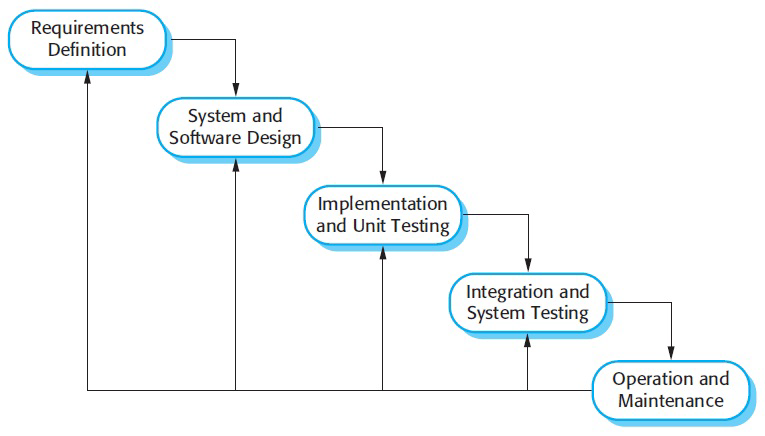
\includegraphics[width=\textwidth]{images/sdlc}
  \caption{Alur SDLC \emph{Waterfall} pada Penelitian}
  \label{fig:sdlc-waterfall}
\end{figure}

Berikut merupakan penjelasan setiap fase beserta implementasinya pada penelitian ini.

\begin{enumerate}
\item \emph{Requirement Definition}

Sommerville mendefinisikan fase ini sebagai proses untuk menetapkan layanan, batasan, dan tujuan sistem melalui konsultasi dengan pengguna yang kemudian didefinisikan secara rinci sebagai spesifikasi sistem. Pada penelitian ini, fase ini mencakup penyebaran survei kepada mahasiswa untuk memahami kondisi pencarian mitra kolaborasi saat ini, hambatan yang dihadapi, serta atribut yang dianggap penting dalam menentukan kecocokan. Seluruh temuan dirumuskan ke dalam kebutuhan fungsional dan nonfungsional modul \emph{People-to-Project} yang menjadi fondasi seluruh tahap berikutnya.

\item \emph{System and Software Design}

Sommerville menjelaskan bahwa fase ini mengalokasikan kebutuhan ke dalam komponen sistem dan menetapkan arsitektur perangkat lunak secara menyeluruh, termasuk identifikasi abstraksi fundamental sistem dan hubungan antarkomponen. Pada penelitian ini, fase ini mencakup perancangan arsitektur sistem, diagram UML, logika \emph{Affinity Based Matching}, serta desain antarmuka modul \emph{People-to-Project}.

\item \emph{Implementation and Unit Testing}

Pada fase ini, Sommerville menjelaskan bahwa desain sistem direalisasikan menjadi program atau unit program, dan setiap unit diuji untuk memastikan kesesuaiannya dengan spesifikasi. Pada penelitian ini, implementasi modul \emph{People-to-Project} mencakup pengembangan fitur pengelolaan profil, mekanisme pencocokan berbasis \emph{Affinity Based Matching}, penyajian hasil rekomendasi dalam bentuk \emph{feed}, tampilan detail profil, dan interaksi dasar antarpengguna. Setelah implementasi selesai dilakukan \emph{unit testing} untuk memastikan setiap fungsi berjalan sesuai spesifikasi.

\item \emph{Integration and System Testing}

Sommerville menjelaskan fase ini sebagai tahap penggabungan seluruh unit program menjadi sistem yang utuh dan pengujian sistem secara menyeluruh untuk memastikan seluruh kebutuhan perangkat lunak telah terpenuhi. Pada penelitian ini, ketiga modul \emph{People-to-People}, \emph{People-to-Project}, dan Team Formation diintegrasikan menjadi satu platform dan diuji secara fungsional untuk memvalidasi kesesuaian sistem dengan spesifikasi yang telah ditetapkan.

\item \emph{Operation and Maintenance}

Sommerville mendefinisikan fase ini sebagai fase terpanjang dalam siklus hidup. Pada fase ini, sistem dipasang dan digunakan secara nyata serta dipelihara dengan memperbaiki kesalahan yang tidak terdeteksi pada fase sebelumnya. Sesuai batasan penelitian ini, fase \emph{Operation and Maintenance} tidak menjadi cakupan pengerjaan tugas akhir.

\end{enumerate}

% --- Sistematika Penulisan ---
\section{Sistematika Penulisan}

Laporan tugas akhir ini disusun dalam tujuh bab dengan struktur sebagai berikut.

\begin{enumerate}
\item Bab I Pendahuluan: membahas latar belakang permasalahan yang melatarbelakangi pengembangan modul rekomendasi \emph{People-to-Project}, rumusan masalah, tujuan penelitian, batasan masalah, metodologi pengerjaan, dan sistematika penulisan laporan.
\item Bab II Studi Literatur: membahas kajian pustaka yang relevan dengan topik penelitian, mencakup konsep kolaborasi mahasiswa, tantangan pencarian mitra kolaborasi, sistem rekomendasi, \emph{rule based matching}, \emph{Affinity Based Matching}, model SDLC Waterfall, serta tinjauan terhadap sistem yang sudah ada.
\item Bab III Analisis: membahas analisis kondisi pencarian mitra kolaborasi mahasiswa saat ini, identifikasi masalah pengguna berdasarkan hasil survei, penurunan kebutuhan dari \emph{user needs} hingga \emph{functional requirement}, serta analisis pemilihan solusi.
\item Bab IV Perancangan Sistem Rekomendasi Modul \emph{People-to-Project}: membahas gambaran umum sistem secara menyeluruh serta perancangan model sistem modul \emph{People-to-Project}, mencakup dekomposisi dan pembagian modul, diagram UML, perancangan arsitektur, perancangan basis data, desain antarmuka, serta perancangan algoritma \emph{Affinity Based Matching}.
\item Bab V Implementasi Modul Rekomendasi \emph{People-to-Project}: membahas proses implementasi modul \emph{People-to-Project} berdasarkan hasil perancangan, mencakup lingkungan implementasi, implementasi setiap \emph{use case}, implementasi antarmuka, implementasi algoritma, dan berkas pendukung lainnya.
\item Bab VI Evaluasi: membahas pengujian sistem yang telah diimplementasikan, mencakup metode pengujian, skenario uji, hasil pengujian fungsional, dan penilaian terhadap kesesuaian sistem dengan rumusan masalah dan tujuan penelitian.
\item Bab VII Kesimpulan dan Saran: membahas kesimpulan dari hasil pelaksanaan tugas akhir berdasarkan evaluasi yang telah dilakukan, serta saran untuk pengembangan sistem lebih lanjut.
\end{enumerate}
